\section{Metodología}

A continuación se explica de manera fundamentada, sobre la base de lo descrito en este documento, la Metodología propuesta. La Metodología General que nuestra empresa, emplea y emplearía para obtener los resultados esperados, en función de los requerimientos.

\subsection{Desarrollo del Proyecto}

La metodología que seguimos, como marco de referencia, para el desarrollo de cualquier proyecto de complejidad media o alta está basada en los procesos de ciclo de ingeniería de software iterativo e incremental, desarrollado, recomendado y normalizado inicialmente por la empresa Rational Software, que hoy es propiedad de IBM, su denominación es Rational Unified Process \textquote{RUP}, 

Además, se usan principios de metodologías como SCRUM y Kanban para mejorar la comunicación con el cliente y la administración de tareas.

Tener una metodología de referencia como RUP, posibilita un profundo y razonado trabajo interdisciplinario, de equipos de profesionales que determinan los casos de uso para cada aplicación. 
Estos casos actúan como el hilo conductor a través de todas las etapas de creación del software del sistema (usando el Lenguaje de Modelado Unificado - UML), 
pues definen las acciones del usuario, los comportamientos de la aplicación y como ésta interactúa con otros programas instalados en los computadores. 
Además de especificar los casos de uso con UML, RUP nos ayuda a construir un plan de integración y evaluación del software, para brindar a los desarrolladores de Jucux y a los usuarios finales la certeza de que la totalidad del producto y cada una de sus partes se construirán como prototipos para ser evaluados y probados antes de su fase de implementación, algo que en SCRUM se llama el MVP (Minimum Viable Product). 

La metodología asegurará que obtengamos un sistema o sistemas menos susceptibles al fallo, y estables arquitectónicamente.

\begin{figure}[htbp]
    \centering
    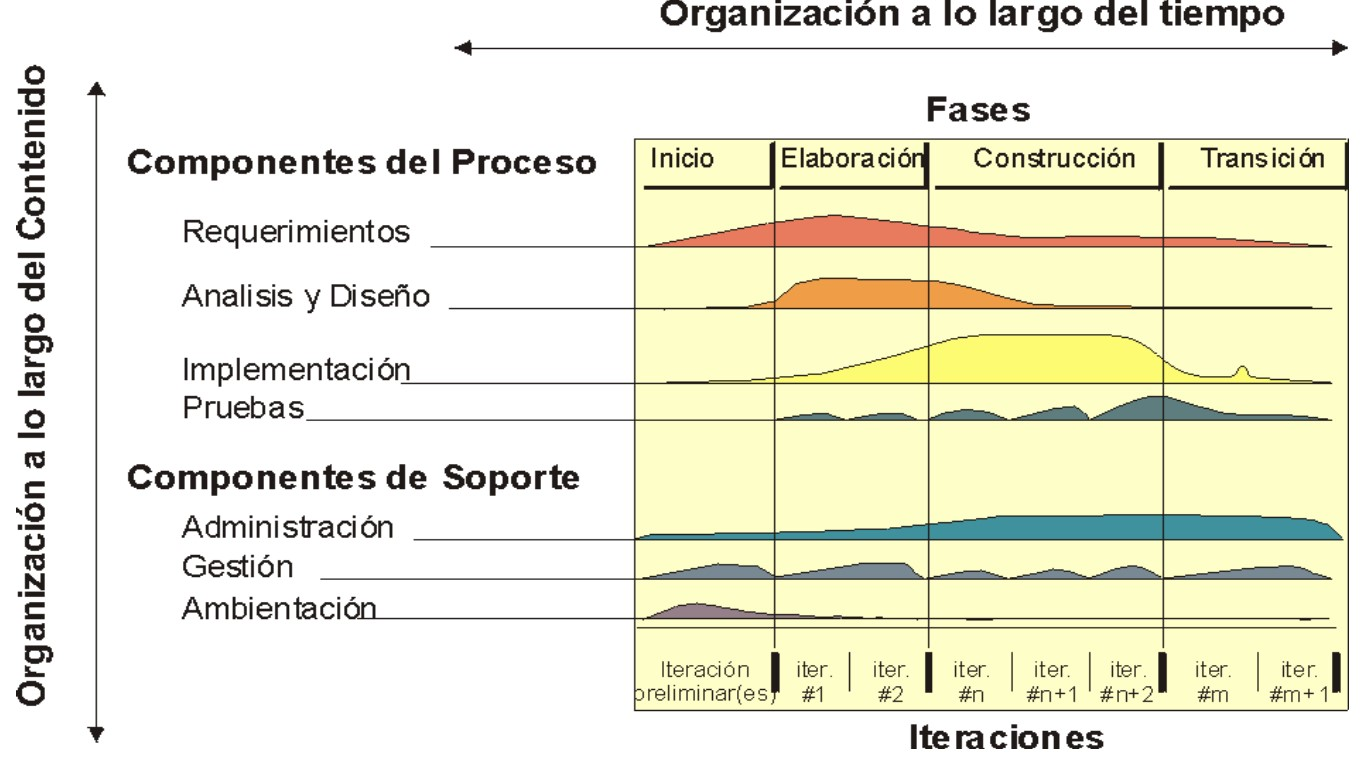
\includegraphics[width=0.7\textwidth]{assets/RUPGRAPH.JPG}
    \caption{Organización del proceso de desarrollo RUP }
    \label{fig:rupgraph}
\end{figure}

Sus características son:

\begin{itemize}
    \item Contiene las mejores prácticas de software desarrolladas por las compañías líderes de la industria.
    \item• Reduce riesgos e incrementa la predictibilidad en el desarrollo del software. • 
    \item Provee una visión y cultura estándar dentro de la organización. • 
    \item Crea y permite utilizar software reusable. • 
    \item Es soportado por herramientas muy efectivas que automatizan cada una de las fases del desarrollo del proyecto de software.
    \item Utiliza el estándar de nomenclatura Unified Modeling Language (UML).
\end{itemize}

